\documentclass[tikz]{standalone}
\usepackage{tikz}
\usetikzlibrary{positioning, graphs}
\usetikzlibrary{graphs.standard}
\begin{document}
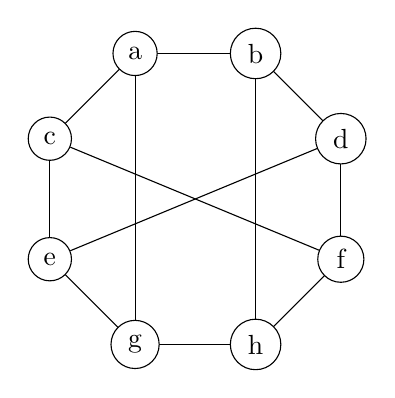
\begin{tikzpicture}
		[vertex/.style={draw,circle,inner sep = 0mm, minimum size = 2mm},
		 edgelabel/.style = {fill = white, inner sep = 0mm, font=\tiny}]

        \graph[clockwise, radius = 2cm, empty nodes, phase=112.5]{subgraph C_n[n = 8, name = A]};

        \node[draw, circle, minimum width=10, fill=white] (a) at (A 1) {a};
        \node[draw, circle, minimum width=10, fill=white] (b) at (A 2) {b};
        \node[draw, circle, minimum width=10, fill=white] (d) at (A 3) {d};
        \node[draw, circle, minimum width=10, fill=white] (f) at (A 4) {f};
        \node[draw, circle, minimum width=10, fill=white] (h) at (A 5) {h};
        \node[draw, circle, minimum width=10, fill=white] (g) at (A 6) {g};
        \node[draw, circle, minimum width=10, fill=white] (e) at (A 7) {e};
        \node[draw, circle, minimum width=10, fill=white] (c) at (A 8) {c};

        \draw (a) -- (g);
        \draw (b) -- (h);
        \draw (c) -- (f);
        \draw (d) -- (e);
\end{tikzpicture}
\end{document}